%\listfiles % List packages used in log file
\documentclass[11pt]{report}
\usepackage[english]{babel} % language selection
\usepackage[utf8]{inputenc} % Accept different input encodings
\usepackage{csquotes}       % Context sensitive quotation facilities
\usepackage[style=apa,
            backend=biber]
            {biblatex}      % APA style bibliography support
\DeclareLanguageMapping{english}{english-apa}    % Language mapping
\addbibresource[datatype=bibtex]{references.bib} % Use a bibtex bibliography file
\usepackage[a4paper,            % Set to a4 paper
            left    = 2.5cm,    % Left paper margin
            right   = 2.5cm,    % Right paper margin
            top     = 2.5cm,    % Top paper margin
            bottom  = 2.5cm     % Bottom paper margin
            ]{geometry}
\usepackage{graphicx}                   % Include graphics
\graphicspath{{./images/}
              {../misc/logo/}}          % Graphics paths
\usepackage{titling}                    % Title page
\usepackage{fancyhdr}                   % Make header end footer
\usepackage{tocloft}                    % Control table of contents, figures, etc
\usepackage{changepage}                 % for the adjustwidth environment
\usepackage[quiet]{fontspec}            % load custom fonts
\usepackage{titlesec}                   % set format per section type
\usepackage{fancyvrb}                   % Sophisticated verbatim text
\usepackage{longtable}                  % Longtable support
\usepackage{booktabs}                   % toprule problem
\usepackage{bookmark}                   % Generate bookmarks
\usepackage{hyperref}                   % Generate links
\usepackage{xcolor}                     % Color for links etc
\usepackage{etoolbox}                   % e-TEX tools for LATEX
\usepackage{caption}                    % Customizing captions in floating environments
\usepackage{subcaption}                 % Support for sub-captions
\usepackage{chngcntr}                   % Change the resetting of counters
\usepackage{float}                      % Improved interface for floating objects
\usepackage[bottom,
            hang,
            flushmargin]
            {footmisc}                  % A range of footnote options
            \usepackage{dirtytalk}
\usepackage{wrapfig}                    % Produces figures which text can flow around
%\usepackage{lipsum}                     % For sample text
\usepackage{enumitem}                   % list support

%%%%%%%%%%%%%%%%%%%%%%%%%%%%%%%%%%%%%%%%
%   Setup main document parameters
%%%%%%%%%%%%%%%%%%%%%%%%%%%%%%%%%%%%%%%%
% Main title
\def \title {Dynamic Network of Speakers}
% Sub title
\def \subtitle {With MQTT}
% Institution
\def \institution {HAN University of Applied Sciences}
% Sub department
\def \subdepartment {Embedded Systems Engineering}
% Author(s)
\author{
    Ingmar Delsink
    \and\\
    Menno van der Graaf
    \and\\
    Brian van Zwam
}
% Publish data
\date{May 2016}
% Version number
\def \version{0.1}

%%%%%%%%%%%%%%%%%%%%%%%%%%%%%%%%%%%%%%%%
%%%%    Styling
%%%%%%%%%%%%%%%%%%%%%%%%%%%%%%%%%%%%%%%%
% Hyperlinks formatting
\hypersetup{
    colorlinks=true,            % Colors the text of links and anchors.
    pdfborderstyle={/S/U/W 1},  % underline links instead of boxes
    linkcolor=[RGB]{50,50,50},  % Color for normal internal links.
    anchorcolor=red,            % Color for anchor text.
    citecolor=red,              % Color for bibliographical citations in text.
    filecolor=magenta,          % Color for URLs which open local files.
    menucolor=red,              % Color for Acrobat menu items.
    runcolor=red,               % Color for run links (launch annotations).
    urlcolor=[RGB]{50,50,50},   % Color for linked URLs.
    bookmarks=true,             % A set of Acrobat bookmarks are written
    bookmarksnumbered=true,     % If Acrobat bookmarks are requested, include section numbers.
    citebordercolor=red,        % The color of the box around citations
    filebordercolor=red,        % The color of the box around links to files
    linkbordercolor=red,        % The color of the box around normal links
    menubordercolor=red,        % The color of the box around Acrobat menu links
    urlbordercolor=red,         % The color of the box around links to URLs
    runbordercolor=red,         % Color of border around ‘run’ links
    pdfinfo={                   % Global PDF info
        Title={\title},
        Subject={\subtitle},
        Author={\theauthor},
        Institution={\institution},
        Subdepartment={\subdepartment},
        Version={\version}
    }
}
% Load custom fonts
\newfontfamily\xolonium[
    Path = {../misc/fonts/xolonium/} ,
    Extension = .otf ,
    UprightFont = *-Regular ,
    BoldFont = *-Bold
    ]{Xolonium}
\newfontfamily\nimbus[
    Path = {../misc/fonts/nimbus-sans-l/} ,
    Extension = .ttf ,
    UprightFont = *_regular ,
    ItalicFont = *_italic ,
    BoldFont = *_bold ,
    BoldItalicFont = *_bold-italic,
    Ligatures = {   % Set Ligature options
       NoCommon,
       NoRequired,
       NoContextual,
       NoHistoric,
       NoDiscretionary,
       TeX
   }
   ]{nimbus-sans-l}
% Footnotes
\renewcommand{\footnotelayout}{
    \footnotesize\nimbus
}

%%%%%%%%%%%%%%%%%%%%%%
%% Table of Content
%%%%%%%%%%%%%%%%%%%%%%
\setlength{\cftbeforetoctitleskip}{0ex} % Set ToC before height
\setcounter{tocdepth}{2}                % Set depth of entries
\setcounter{secnumdepth}{2}             % Section number dept (subsection)
\addtocontents{toc}{                    % Add "Page" on top of ToC #
    ~\hfill{\xolonium Page}\par
}
% Indent size {<entry>}{<indent>}{<numwidth>}
\cftsetindents{chapter}{0em}{2.5em}
\cftsetindents{section}{1em}{2.5em}
\cftsetindents{subsection}{1.8em}{3.2em}
\cftsetindents{subsubsection}{6.0em}{5em}
\cftsetindents{paragraph}{7.0em}{5.0em}
\cftsetindents{subparagraph}{12.0em}{6.0em}
% sectional unit title format per section
\renewcommand{\cfttoctitlefont}{\Huge\xolonium}     % ToC title
\renewcommand{\cftchapfont}{\normalsize\xolonium}   % chapter
\renewcommand{\cftsecfont}{\normalsize\nimbus}      % section
\renewcommand{\cftsubsecfont}{\normalsize\nimbus}   % subsection
% Page number format per section
%% Skip distance
\renewcommand\cftchapafterpnum{\vskip6pt}   % chapter page
\renewcommand\cftsecafterpnum{\vskip6pt}    % section page
\renewcommand\cftsubsecafterpnum{\vskip6pt} % subsection page
%% Font
\renewcommand{\cftchappagefont}{\small\xolonium}  % chapter page font
\renewcommand{\cftsecpagefont}{\small\nimbus}     % section page font
\renewcommand{\cftsubsecpagefont}{\small\nimbus}  % subsection page font
%%%%%%%%%%%%%%%%%%%%%%
%% List of Tables
%%%%%%%%%%%%%%%%%%%%%%
\setlength{\cftbeforelottitleskip}{0ex} % Set LoT before height
\setcounter{lotdepth}{2}                % Set depth of entries
\addtocontents{lot}{                    % Add "Page" on top of LoT #
    ~\hfill{\xolonium Page}\par
}
% sectional unit title format per section
\renewcommand{\cftlottitlefont}{\Huge\xolonium}     % LoT title
\renewcommand{\cfttabfont}{\normalsize\nimbus{Table }}  % LoT entries
\setlength{\cfttabnumwidth}{4em}  % Modify number width in LoT
% Page number format per section
%% Skip distance
\renewcommand\cfttabafterpnum{\vskip6pt}        % figure page
%% Font
\renewcommand{\cfttabpagefont}{\small\nimbus}   % figure page font
%%%%%%%%%%%%%%%%%%%%%%
%% List of Figures
%%%%%%%%%%%%%%%%%%%%%%
\setlength{\cftbeforeloftitleskip}{0ex} % Set LoF before height
\setcounter{lofdepth}{2}                % Set depth of entries
\addtocontents{lof}{                    % Add "Page" on top of LoF #
    ~\hfill{\xolonium Page}\par
}
% sectional unit title format per section
\renewcommand{\cftloftitlefont}{\Huge\xolonium} % LoF title
\renewcommand{\cftfigfont}{\normalsize\nimbus{Figure }}  % LoF entries
\setlength{\cftfignumwidth}{4em}  % Modify number width in LoF

% Page number format per section
%% Skip distance
\renewcommand\cftfigafterpnum{\vskip6pt}        % figure page
%% Font
\renewcommand{\cftfigpagefont}{\small\nimbus}   % figure page font
%%%%%%%%%%%%%%%%%%%%%%
%% Bibliography
%%%%%%%%%%%%%%%%%%%%%%
\def\bibfont{\nimbus}   % Set font

%%%%%%%%%%%%%%%%%%%%%%
%% Format per section
%%%%%%%%%%%%%%%%%%%%%%
% Chapter
\titleformat{\chapter}
    [hang] % shape
    {\Large\xolonium} % format
    {\thechapter} % label
    {1.5em} % horizontal sep between label and title body
    {} % before-code
    [] % after-code
\titlespacing{\chapter}
    {0em}   % left spacing
    {0ex}   % before spacing
    {3ex}   % after spacing
% Section
\titleformat{\section}
    [hang] % shape
    {\Large\xolonium} % format
    {\thesection} % label
    {2em} % horizontal sep between label and title body
    {} % before-code
    [] % after-code
\titlespacing{\section}
    {0em}   % left spacing
    {2ex}   % before spacing
    {2ex}   % after spacing
% Subsection
\titleformat{\subsection}
    [hang] % shape
    {\normalsize\xolonium} % format
    {\thesubsection} % label
    {2.5em} % horizontal sep between label and title body
    {} % before-code
    [] % after-code
\titlespacing{\subsection}
    {0em}   % left spacing
    {2ex}   % before spacing
    {1ex}   % after spacing
% Subsubsection
\titleformat{\subsubsection}
    [hang] % shape
    {\xolonium} % format
    {\thesubsubsection} % label
    {3em} % horizontal sep between label and title body
    {} % before-code
    [] % after-code
\titlespacing{\subsubsection}
    {0em}   % left spacing
    {2ex}   % before spacing
    {1ex}   % after spacing
% Paragraph
\titleformat{\paragraph}
    [hang] % shape
    {\normalfont\normalsize\xolonium\color{cyan}} % format
    {\theparagraph} % label
    {1em} % horizontal sep between label and title body
    {} % before-code
    [] % after-code
\titlespacing{\paragraph}
    {0em}   % left spacing
    {2ex}   % before spacing
    {1ex}   % after spacing

%%%%%%%%%%%%%%%%%%%%%%
%% Format captions
%%%%%%%%%%%%%%%%%%%%%%
% Tables
\renewcommand{\thetable}{\arabic{table}}        % numbering:  1, 2 etc.
\DeclareCaptionFormat{tabcapfont}
    {\nimbus \small\textit{\textbf{#1#2}}#3}    % caption format
\captionsetup[table]{format=tabcapfont}         % set defined caption
\counterwithin{table}{section}
% Sub Tables
\renewcommand{\thesubtable}{\alph{subtable}}   % a, b etc.
% Figures
\renewcommand{\thefigure}{\arabic{figure}}      % numbering:  1, 2 etc.
\DeclareCaptionFormat{figcapfont}
    {\nimbus \small\textit{\textbf{#1#2}}#3}    % caption format
\captionsetup[figure]{format=figcapfont}        % set defined caption
\counterwithin{figure}{chapter}
% Sub figures
\renewcommand{\thesubfigure}{\alph{subfigure}}  % a, b etc.
%%%%%%%%%%%%%%%%%%%%%%
%% Header and Footer
%%%%%%%%%%%%%%%%%%%%%%
\pagestyle{fancy}                       % Set default style
\fancyhf{}                              % Clear all header and footer fields
\lhead{\nimbus\title}                   % Left head
\rhead{\nimbus\nouppercase\leftmark}    % Right head
\lfoot{\nimbus\thedate}                 % Left foot
\rfoot{\nimbus\thepage}                 % Right foot
% Redefine the plain page style
\fancypagestyle{plain}{ % Used at start of chapter
    \fancyhf{} % clear all header and footer fields
    \lhead{\nimbus\title}
    \rhead{\nimbus\nouppercase\leftmark}
    \lfoot{\nimbus\thedate}
    \rfoot{\nimbus\thepage}
}

%%%%%%%%%%%%%%%%%%%%%%
%% Lists
%%%%%%%%%%%%%%%%%%%%%%
\newenvironment{shortlist}
{ \begin{itemize}
    \setlength{\itemsep}{0pt}
    \setlength{\parskip}{0pt}
    \setlength{\parsep}{0pt}     }
{ \end{itemize}                  }

%%%%%%%%%%%%%%%%%%%%%%%%%%%%%%%%%%%%%%%%
%%%%    Start document
%%%%%%%%%%%%%%%%%%%%%%%%%%%%%%%%%%%%%%%%
\begin{document}
    \nimbus % Set global font

    
\begin{titlepage}
    \begin{center}
        \Huge
        \textbf{\xolonium\title}
        \rule{\linewidth}{0.08ex} \\[0.5ex]
        \LARGE
        \subtitle

        \vspace{2ex}
        \begin{figure}[h]
            \centering
            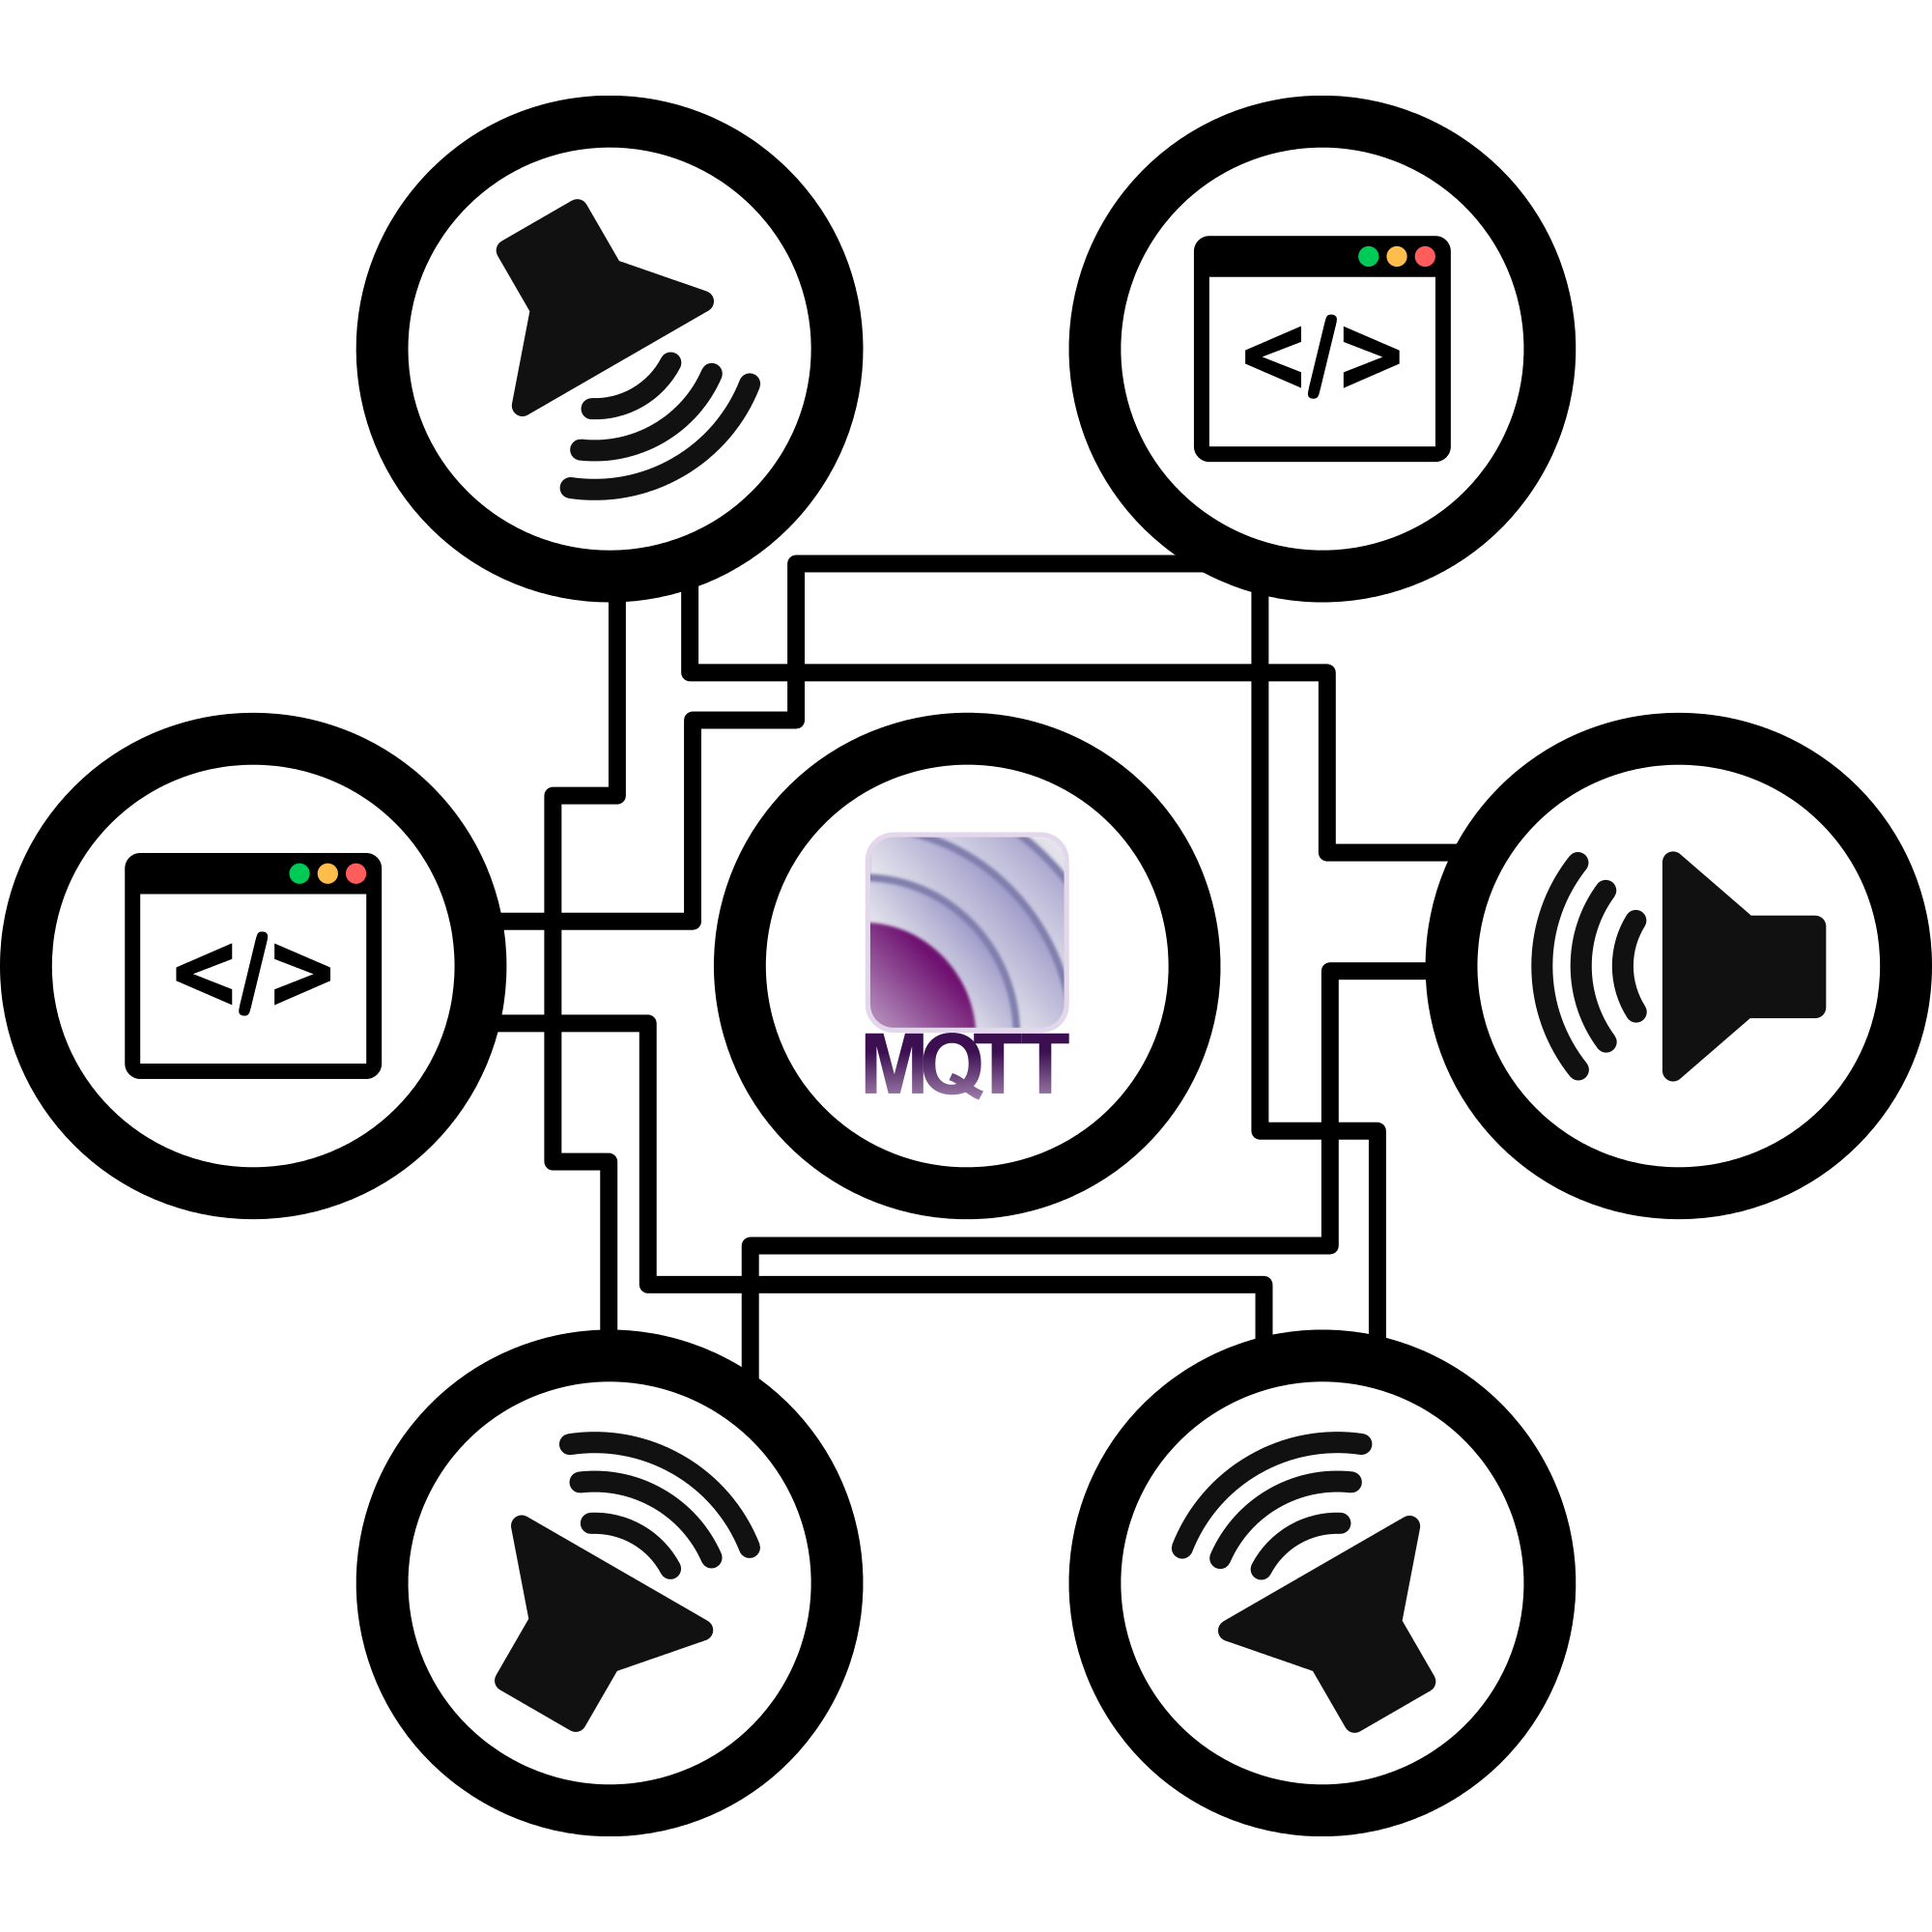
\includegraphics[height=.4\paperheight, keepaspectratio]{dynamic_network_of_speakers}
        \end{figure}


        \vspace{4ex}

        \small\begin{adjustwidth}{22em}{}
            % Author(s)
            \theauthor

            \vspace{1ex}
            % Institution
            \institution

            % Subdepartment
            \subdepartment

            \vspace{1ex}
            \thedate

            v\version
        \end{adjustwidth}
    \end{center}
\end{titlepage}
    % Include the title page

    \chapter*{Summary}              % Summary
    \label{chap:Summary}
    Summary about the project and things achieved.

\section*{Example image}
This image is an example.

\begin{figure}[h]
    \centering
    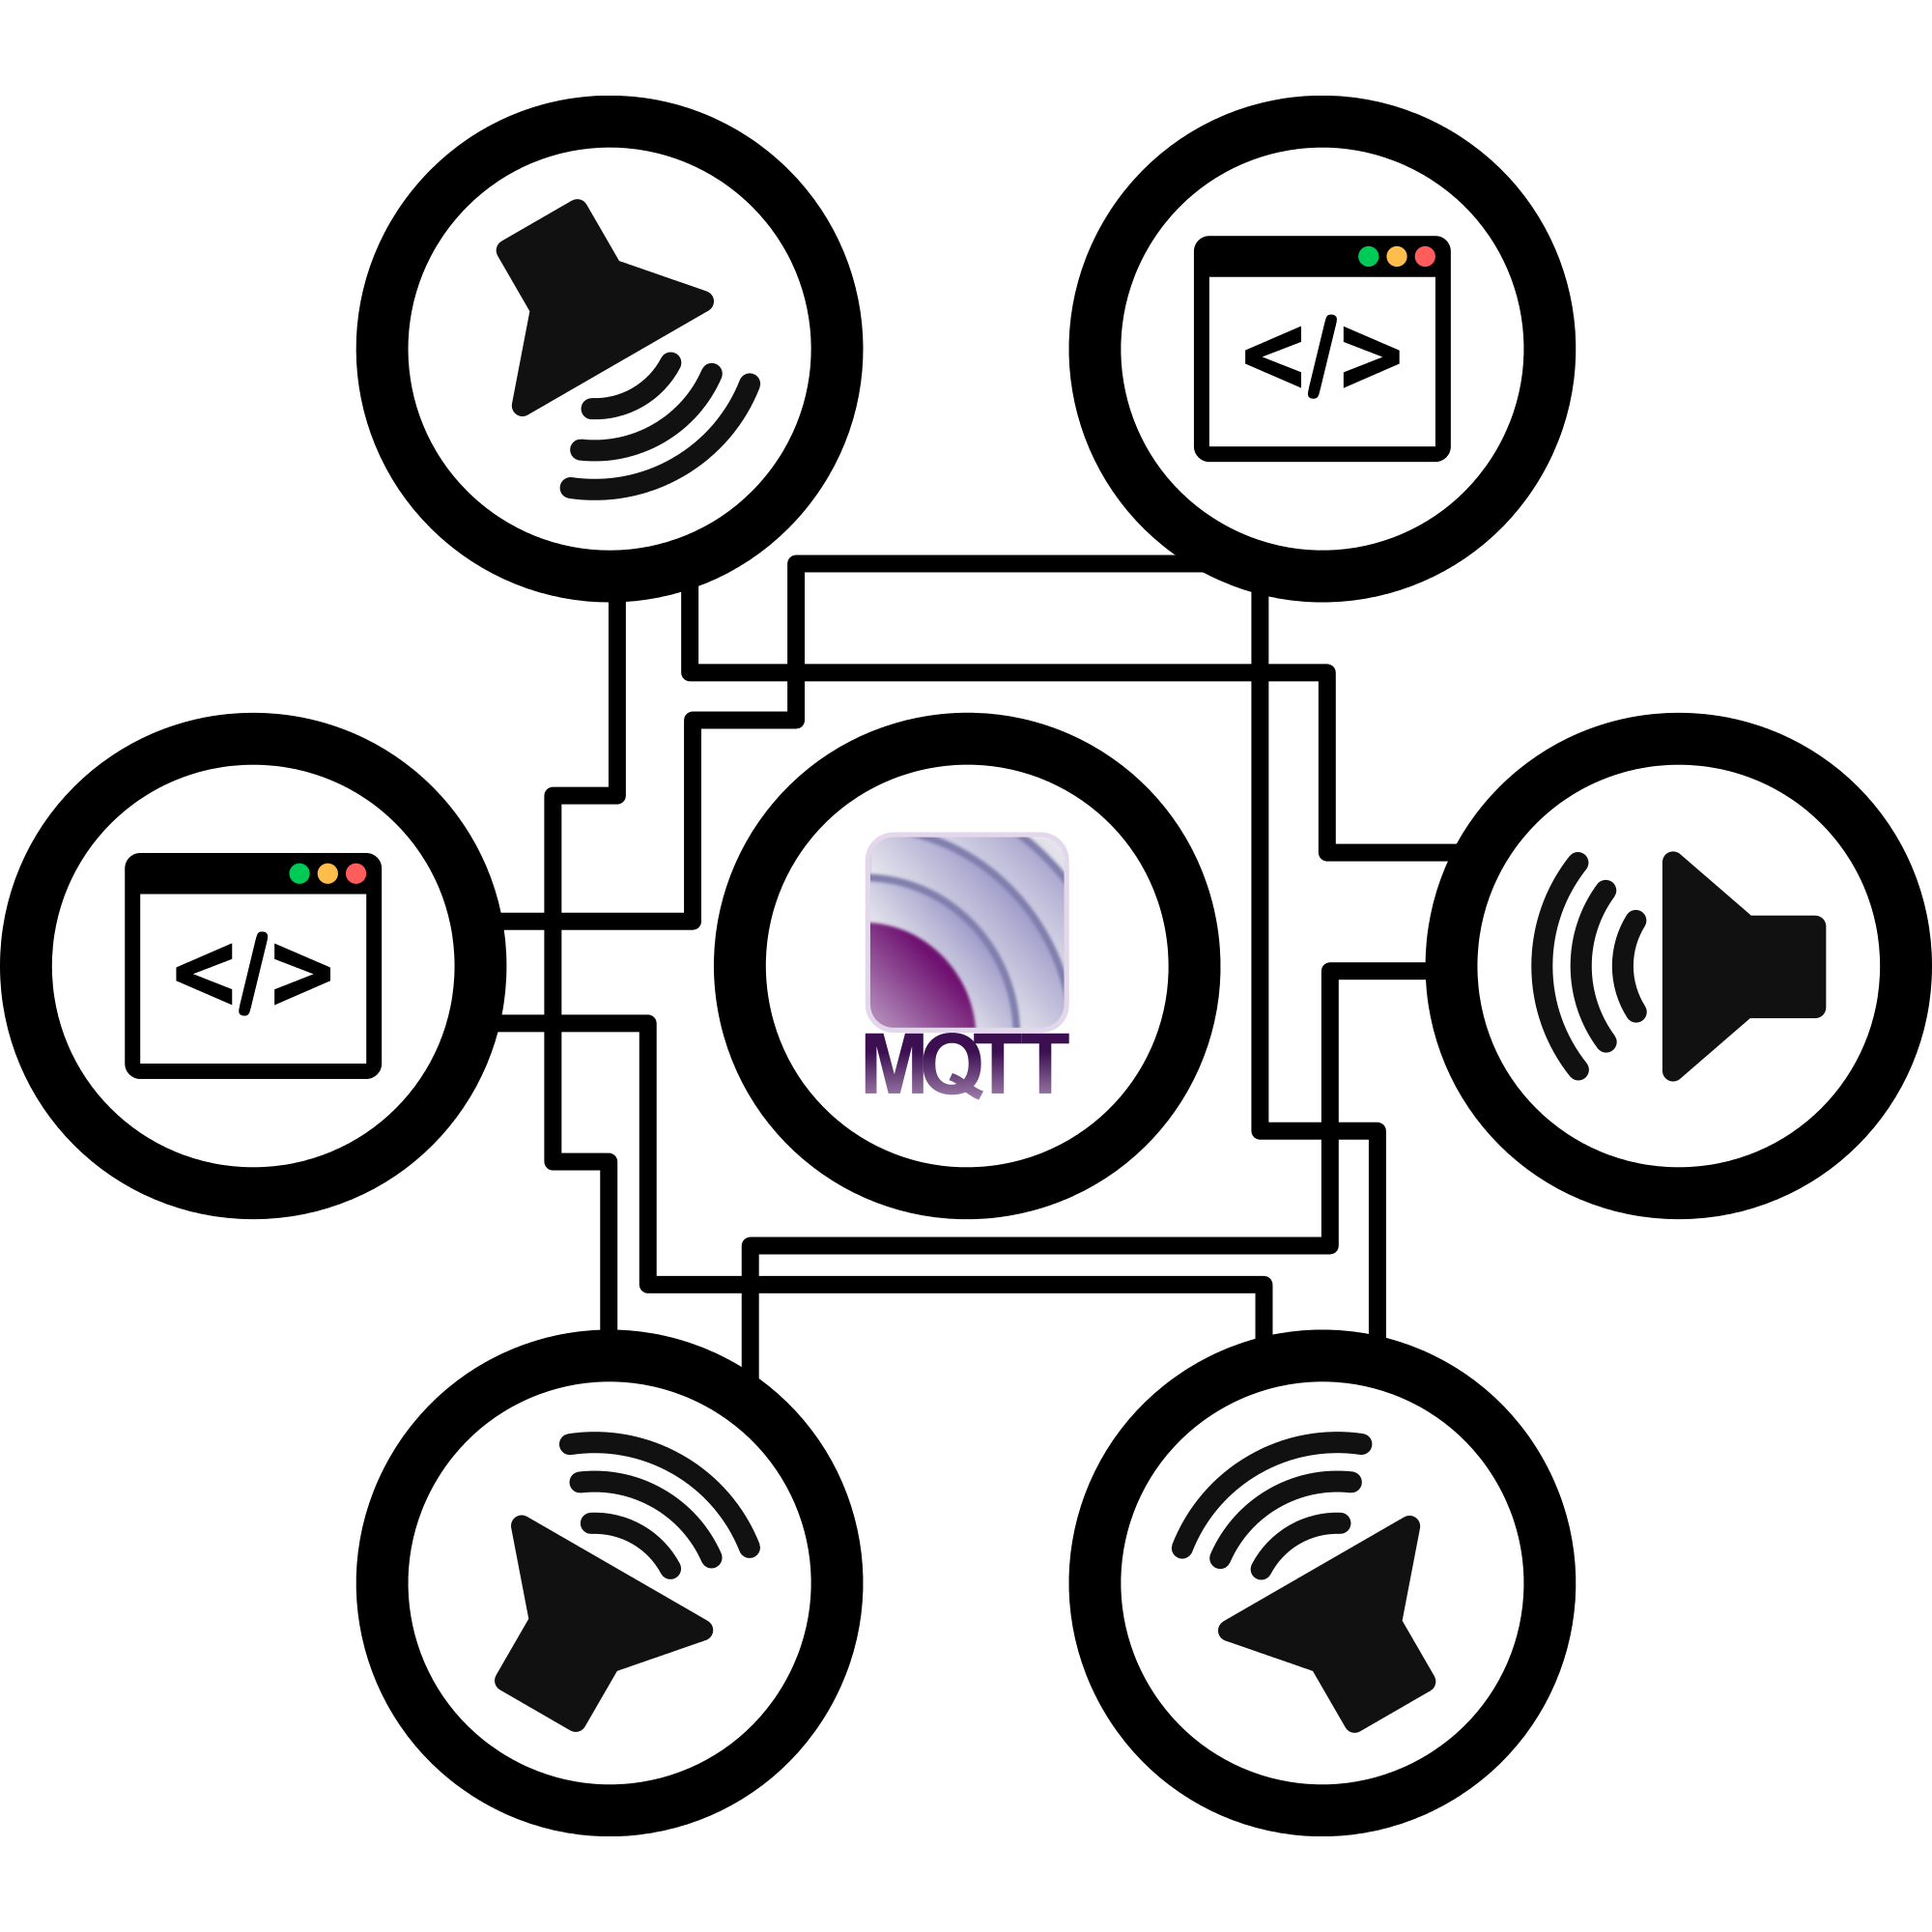
\includegraphics[height=5cm]{dynamic_network_of_speakers}
\end{figure}

\section*{Example citation and URL}
On \href{https://en.wikibooks.org/wiki/LaTeX/Bibliography_Management#Standard_templates}{\textbf{this}} page are examples for the use of APA refrences. \cite{BiberTemplates}.


    \clearpage
    \renewcommand{\contentsname}{Table of Contents} % Set title
    \tableofcontents                % Generate and include a table of contents

    \chapter{Introduction}          % Introduction
    \label{chap:Introduction}
    % README is a good enough introduction

    % Convert readme from markdown to LaTeX
    \immediate\write18{
        pandoc                              % Converter
        ../README.md                        % Source
        -f markdown -t latex                % Type specification
        -o build/readme.tex                 % Destination/output
    }
    \input{./build/readme.tex} % Include generated file
    \vspace{5ex}
    \input{../LICENSE} % Include license file

    \chapter{Topics}                % Topic spec sheet
    \label{chap:Topics}
    Introduction and explanation about the topics used in this project.

    % Convert topic spec sheet from markdown to LaTeX
    \immediate\write18{
        pandoc                              % Converter
        ./topic_specification.md            % Source
        -f markdown -t latex                % Type specification
        -o build/topic_specification.tex    % Destination/output
    }
    \input{./build/topic_specification.tex} % Include generated file

    \chapter{Client}                % Client
    \label{chap:Client}
    In this chapter the client and it's functions are described. The Client exists of the following subsystems:
\begin{shortlist}
    \item MQTT
    \item Message/Config Parser
    \item Audio driver
    \item Relative Weight Factor
    \item Logger
\end{shortlist}

The aforementioned parts will be described in the following sections.

\section{MQTT}

The client uses the \href{http://mosquitto.org/}{Mosquitto MQTT C++ library}.
This is an open source message broker that implements the MQTT protocol versions 3.1 and 3.1.1.
MQTT is a publish-subscribe based \say{light weight} messaging protocol for use on top of the TCP/IP protocol.
It is designed for connections with remote locations where a \say{small code footprint} is required or the network bandwidth is limited.
This makes it suitable for \say{Internet of Things} messaging.

The client and the website use topics to communicate. The topics for the communication are described in the previous chapter.
The DNS class has a public inheritance of the Mosquito class.
This means all public and protected members of the Mosquitto class can be accessed by the DNS class.
The private members cannot directly accessed by DNS class. In the DNS class the Mosquitto functions are been overwritten by DNS's own implementation.
The Mosquitto functions are automatically called by the Mosquitto library.

If the client is executed the Mosquitto library calls the function
\textbf{ on connect}. This function published the client-id in the \textbf{online topic } and subscribe itself on the following topics:
\small{
\begin{itemize} [noitemsep, nolistsep]
	\item \textbf {request online}
	\item \textbf {request client data}
	\item \textbf {clients data}
	\item \textbf {music volume}
	\item \textbf {music status}
	\item \textbf {music sources}
\end{itemize}
}

If the client is stopped or disconnected the Mosquitto library calls the function \textbf {on disconnect}. This function published the client-id in the \textbf {offline topic}.\\

When the client is running and has excuted the function \textbf {on connect}. He waits on a message from a subscribed topic. If there appears a message, the function \textbf {on message} is called. This function has as parameters a mosquitto message struct. This contains:
\small{
\begin{itemize} [noitemsep, nolistsep]
	\item \textbf {int mid}
	\item \textbf {char *topic}
	\item \textbf {void* payload}
	\item \textbf {int payloadlen}
	\item \textbf {int qos}
	\item \textbf {bool retain\\}
\end{itemize}
}

In the function is watched on which topic a message is send. This is done by compare the \textbf {char *topic} of the mosquitto message struct with the defined topic described in chapter 2. When there is a match, a action is carried out.\\

MQTT has a funcion that is called \textbf {last will}. This function is called when a client abruptly disconnected and published his last will message. This can means that the client crashed, hasn't a connection to the broker or something else. In the client this function is implemented and the client will publish his message to the \textbf {offline} topic.

\section{Message/Config Parser}

Almost all the messages that are been send in this application are in \href{http://www.json.org/}{JSON string format}. In C++ this is a bit difficult because the native language doesn't include a JSON Parser. In the client the \href{https://github.com/Zguy/Jzon}{library JZON} is used to parse the JSON string formats.\\

The client must be provided with a file with data in JSON format to be used to initialize the client. The data that can be specified is:
\small{
\begin{itemize} [noitemsep, nolistsep]
	\item \textbf {Names}
	\item \textbf {Log info}
	\item \textbf {Prefixs}
	\item \textbf {Brokers}
	\item \textbf {Topics\\}
\end{itemize}
}
With this it's possible to define the data mentioned above in the config file and it can be used to initialize the clients and the website. The benefits of doing this is that you only have to change the config file and everything still works instead of changing every client individually.

\section{Relative Weight Factor}
\label{sec:client_relative_weight_factor}

This system is based on a virtual object that will create sound like it is in some place in 2D space.
This library calculates the volume level that a speaker needs to be in comparison with all the other speakers.

\subsection{The problem}
\label{sub:client_rwf_the_problem}

The explain the inner workings lets look at an example.

In figure \ref{fig:client_rwf_center} is a simple setup. Two speakers, a virtual object that \say{creates} the sound and the real life user that listens to this.
The speakers are the actual devices that are creating the sound.
What the goal of these speaker is, is to reenact the sound that comes out of a speaker at such a sound level that the user is thinking that the sound comes from a certain place.
In the aforementioned figure, it is clear that the sound levels need to be of the same volume.
That way, the user thinks that the sound at that place is equally as loud, so it is the center of the volume.
\begin{figure}[H]
    \centering
    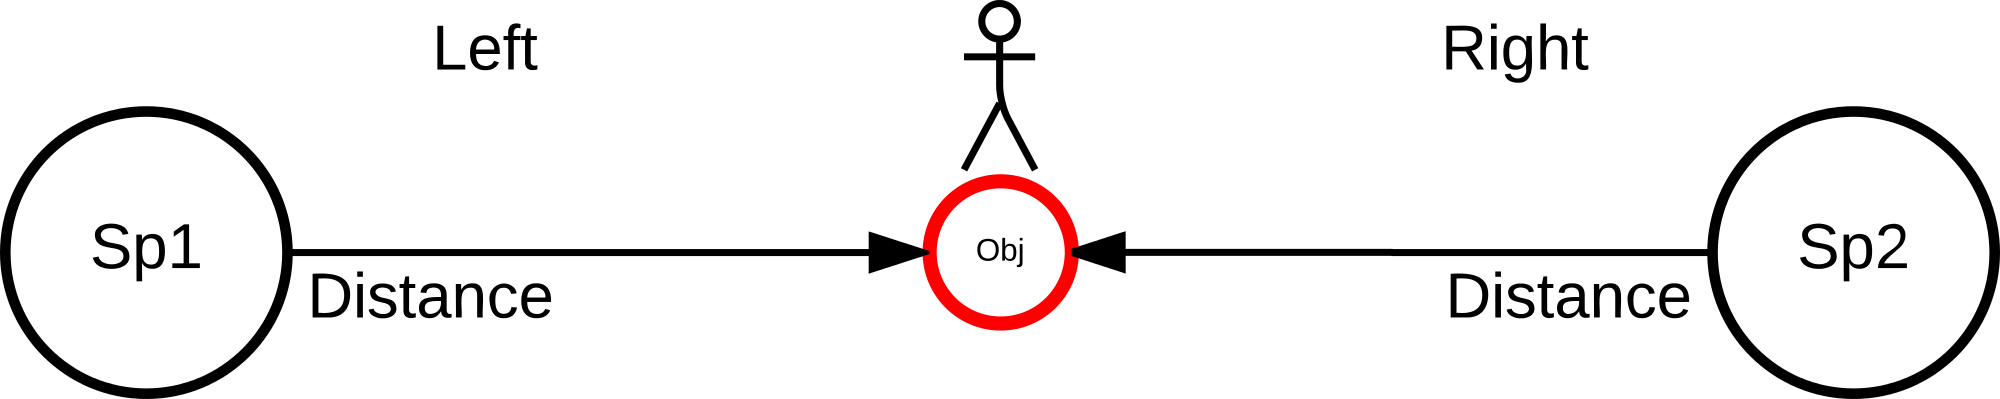
\includegraphics[width=.8\textwidth]{client_rwf_center}
    \caption{Virtual object at center}
    \label{fig:client_rwf_center}
\end{figure}

In figure \ref{fig:client_rwf_offset} is the next example. Now the virtual object is at an offset from the user.
you would normally say that \say{Sp1} has a shorter distance and \say{Sp2} has a greater distance.
To compensate, \say{Sp2} needs to be harder then \say{Sp1}. Let's think about this for a minute.
If the user is standing in the middle and \say{Sp2} is playing harder then \say{Sp1}.
This means that the \say{Right} side produces more sound then the \say{Left} side.
The user would hear more sound comming from the \say{Right} side, so the user would think that the sound comes from the \say{Right} side.

\begin{figure}[H]
    \centering
    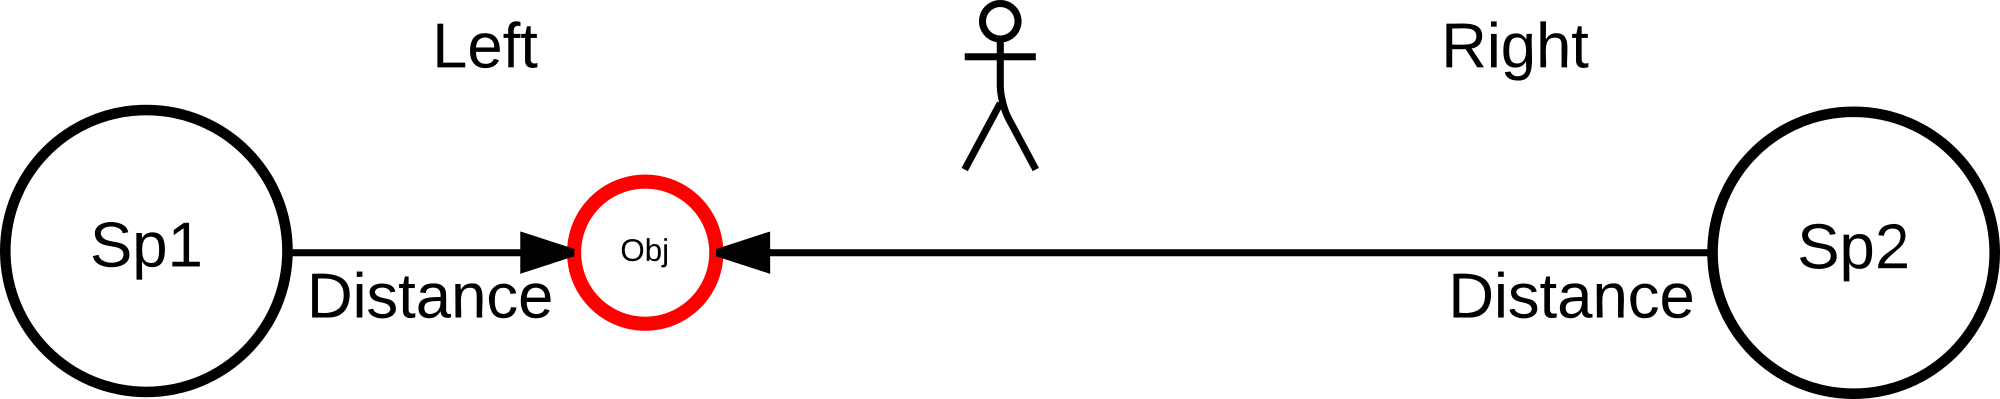
\includegraphics[width=.8\textwidth]{client_rwf_offset}
    \caption{Virtual object at offset}
    \label{fig:client_rwf_offset}
\end{figure}

In conclusion the speaker where the object is closed to, needs to produce the most sound.

\subsection{Calculating value}
\label{sub:client_rwf_calculating_value}

\begin{spreadtab}{{tabular}{ l | r || r l l | r l l }}
    @Speaker    & @Distance                         & @\multicolumn{3}{c|}{Inverse distance}& @\multicolumn{3}{c}{Calculated Value} \\
    @A          & 1                                 & :={b5}&-:={b2}&= :={b5-b2}            &  :={e2}&*:={e10}&= :={round(e2*(e9/e5), 0)} \\
    @B          & 2                                 & :={b5}&-:={b3}&= :={b5-b3}            &  :={e3}&*:={e10}&= :={round(e3*(e9/e5), 0)}\\
    @C          & 3                                 & :={b5}&-:={b4}&= :={b5-b4}            &  :={e4}&*:={e10}&= :={round(e4*(e9/e5), 0)}\\
    @Total:     & sum(b2:b4)                        &       &       &= :={sum(e2:e4)}       &  \\ \hline
                &                                   &       &       &                       &  \\
    @\multicolumn{2}{r ||}{Head}                    & 100   &       &                       &  \\
    @\multicolumn{2}{r || }{Tail}                   & 0     &       &                       &  \\
    @\multicolumn{2}{r || }{Volume steps}           & :={c7}&-:={c8}& = :={c7-c8}           & \\
    @\multicolumn{2}{r || }{Value per volume step}  & :={e9}&/:={e5}& = :={round(e9/e5, 2)} & \\
\end{spreadtab}


    \chapter{Website}               % Website
    \label{chap:Website}
    In this chapter the website and it's functions are described.
Furthermore, there will be some explanation about the logic that drives the website.

\section{Reason of existence}
The website is the place where the online speakers and objects are manipulated.
The idea of the website is to enable the user to simply drag and drop speakers/objects with platform independency in mind.
The website had to be simple, easy to use and not dependent on some kind of webserver.
So the website has to be portable\footnote{Platform independent, eg usable on Linux, Windows, etc...}.
For this reason the website's main logic is made in JavaScript and The layout with simple HTML and CSS.
With this implementation most web browser's can open the website, the \textit{index.html} file, and see the site and online speakers.

\section{Challenges}
Some challenges that where faced when making this website.

\subsection{MQTT with web sockets}
This website needs to connect to an MQTT broker.
Because of the rule of platform independency and portability, some kind of connectivity with JavaScript is needed.
Enter the world of web sockets! For this project, the \href{https://github.com/eclipse/paho.mqtt.javascript}{Paho JavaScript Client} is used.
The Paho JavaScript Client is an MQTT browser-based client library written in JavaScript that uses Web Sockets to connect to an MQTT Broker.
This implementations still has some limits\footnotemark, but for this project it was doing it's job quite well.
\footnotetext{When dealing with non Unicode characters, the Paho client will crash. This was addressed apparently in some fork of the client, but not in this implementation.}

\subsection{Website flow}
In figure \ref{fig:website_flow} is the startup and flow sequence of the website displayed.
When the site comes online, the unknown dataset\footnotemark first has to be rebuild.
\footnotetext{The dataset is all the online clients with all the objects and their information. See \hyperref[clients]{clients} of the \hyperref[chap:Topics]{topics chapter}}

\begin{figure}[H]
    \centering
    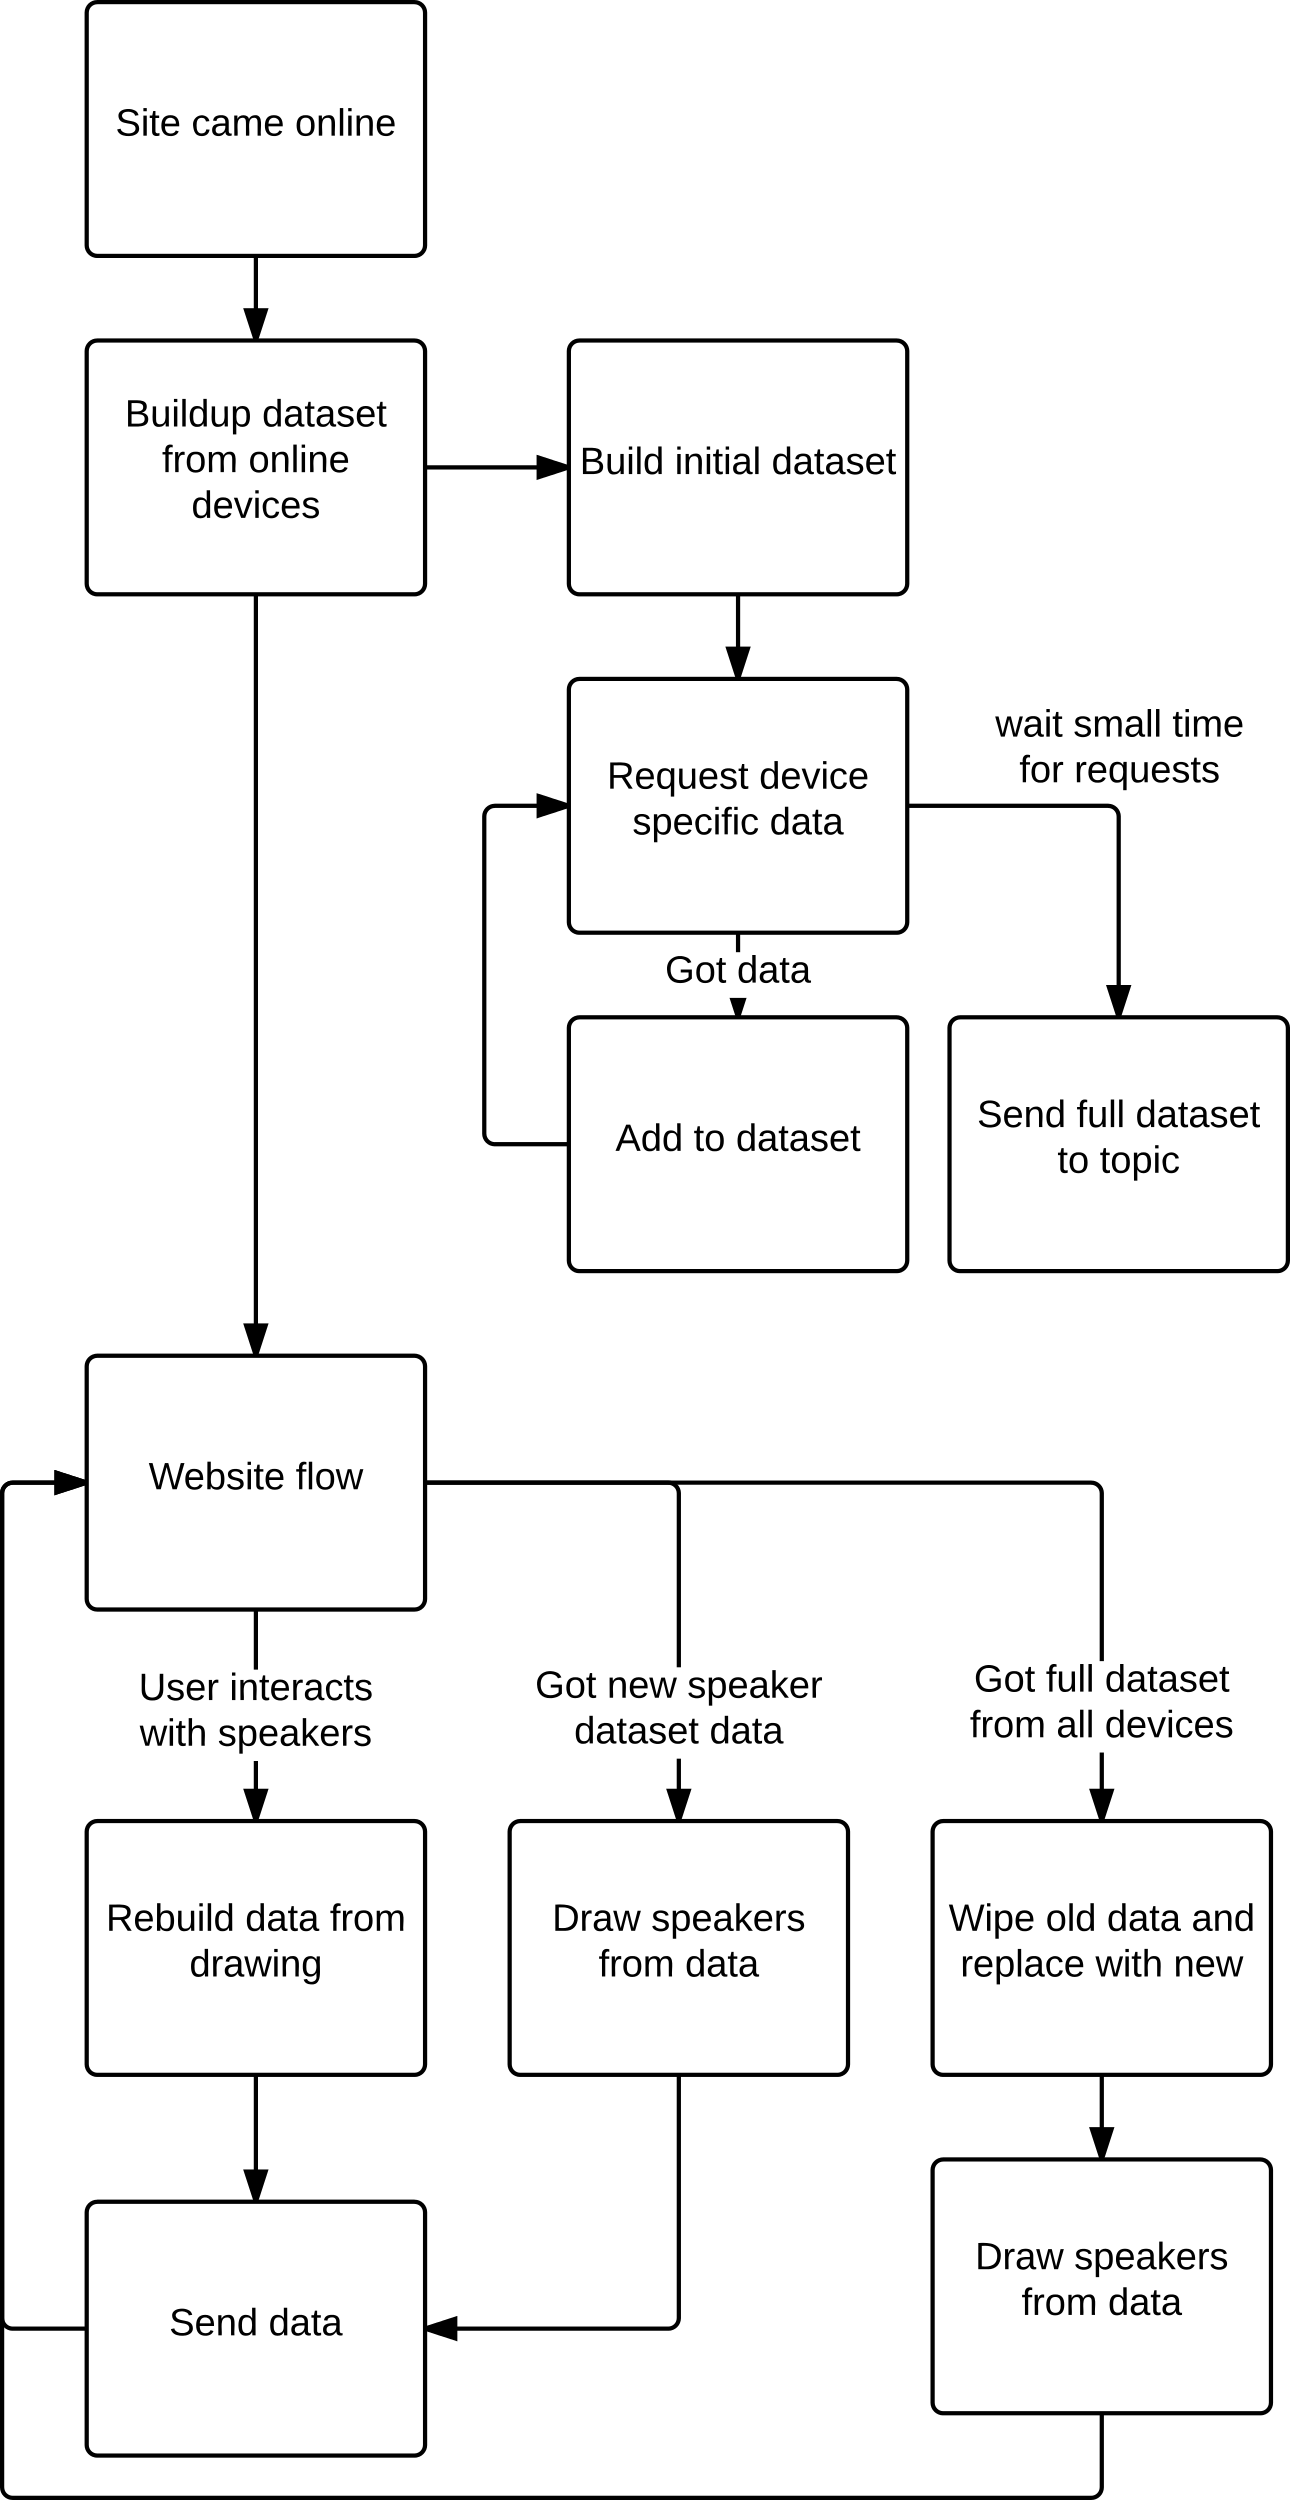
\includegraphics[height=.5\paperheight]{website_flow}
    \caption{The flow of the website}
    \label{fig:website_flow}
\end{figure}

After this initialization, the website is in it's main \say{\textit{flow}}. From here the site has three possibility's:
\begin{shortlist}
    \item User interacts with the drawing (speakers/objects)
    \item Site got new speaker data (from a single speakers)
    \item Site got complete new dataset
\end{shortlist}
In the \hyperref[chap:Topics]{topics chapter}, are the topics defined that are used to send and receive the data to and from all the devices.

\subsection{Draw and synchronize objects}
To draw and synchronize the drawn speakers/objects, there are three features needed.
One that will draw all the available speakers and objects from the dataset,
one that will generate the dataset from the drawn objects and speakers
and a way of synchronizing this data between website and speaker.

\subsubsection{Draw speakers from data}
To draw the speakers and objects, the dataset of all speakers and objects is needed.
This data holds the relations between the speakers and all the objects.
As seen in figure \ref{fig:website_draw_from_data}, it will simply be a looping scheme.
In this diagram, a somewhat crude software architecture is demonstrated.
The drawing is started from an object, and with all the data that is known, the rest is drawn.

Because this is a simple 2D field, all the drawn speakers, will contain all the drawn objects.
I.e. if there are two objects(obj1, obj2) and two speakers(sp1, sp2), sp1 will contain the distance and angle from sp1 to obj1 and obj2.
Sp2 in this example will also have this data, not the same values of course, but it will have the distance and angle from sp2 to obj1 and obj2.
With this knowledge, it is only needed to draw an object or speaker once.
So if a object is drawn, and another speaker has that object, the object doesn't need to be redrawn.

\begin{figure}[H]
    \centering
    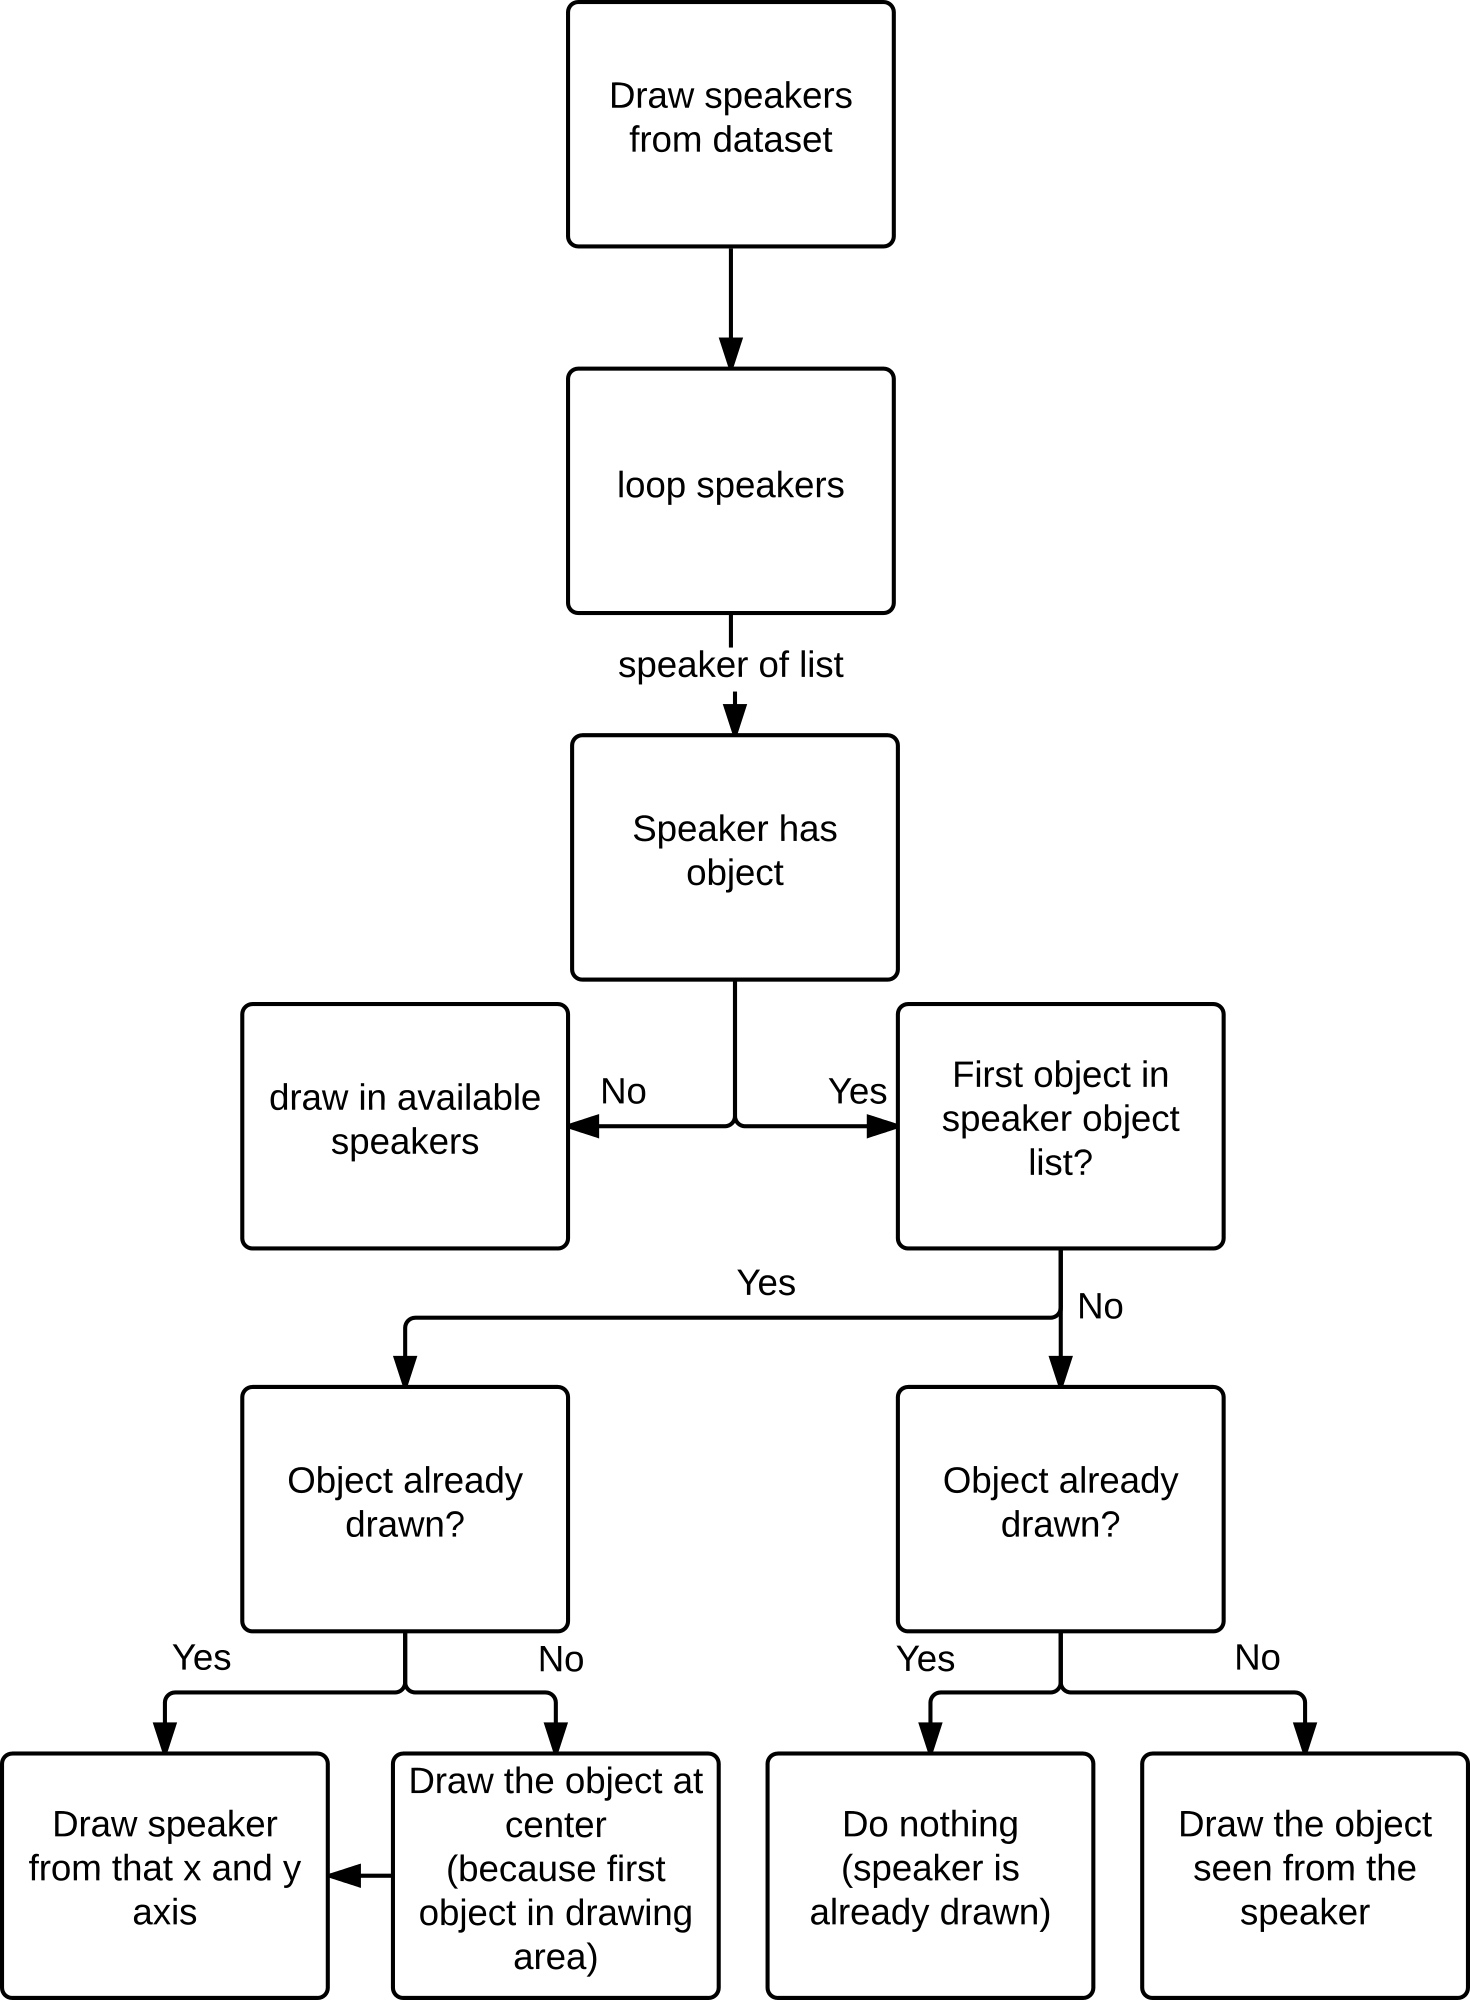
\includegraphics[height=.5\paperheight]{website_draw_from_data}
    \caption{Draw speakers and objects from the dataset}
    \label{fig:website_draw_from_data}
\end{figure}

\subsubsection{Generate dataset from drawing}
This feature has a simple task.
Loop all speakers and calculate all the distances and angles from speaker to the objects.
Figure \ref{fig:website_make_data_from_drawing} describes this quite well.

\begin{figure}[H]
    \centering
    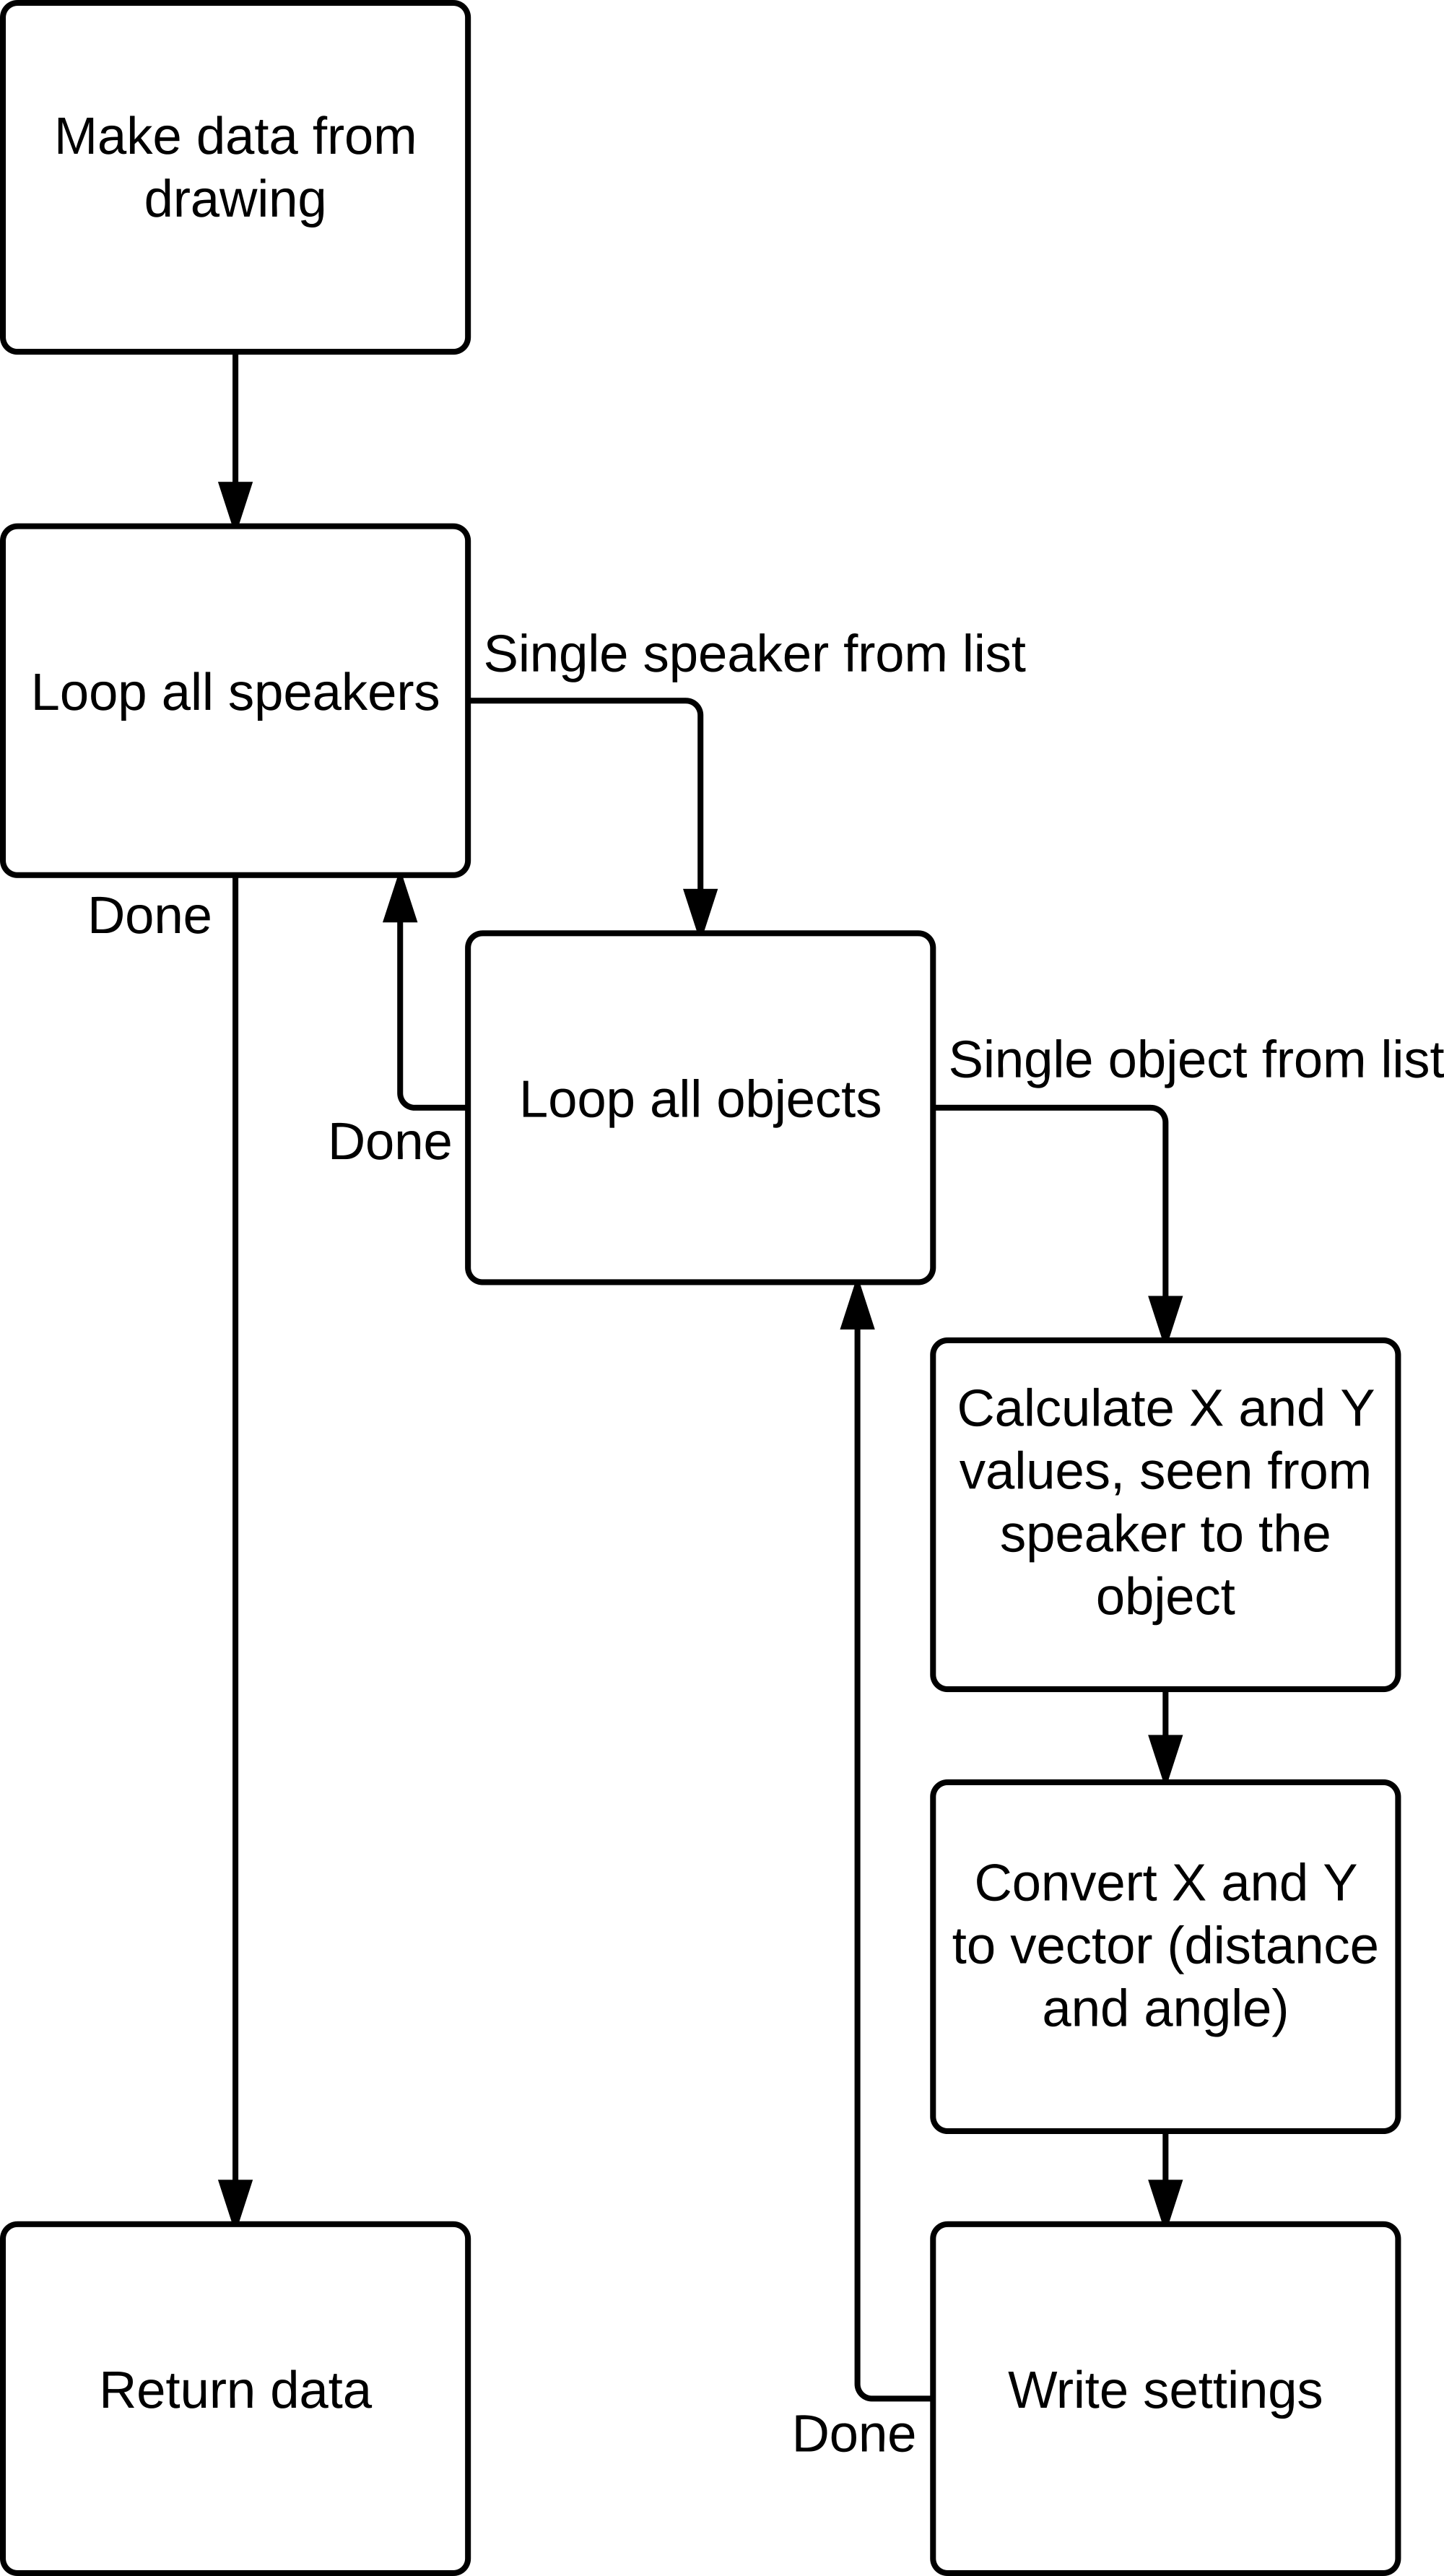
\includegraphics[height=.5\paperheight]{website_make_data_from_drawing}
    \caption{Generate the dataset from the drawing}
    \label{fig:website_make_data_from_drawing}
\end{figure}

\subsubsection{Synchronization}
The last part is the synchronization. This is used for a synchronization between two or more websites and clients.
The dataset is generated.
The moment this is send to a topic, the other websites, not the one sending, will use this data to redraw the speakers and objects.
One extra topic is used in this system specific for the website.
The moment, a website sends this data, it also sends the x and y offset of the first drawn object.
This way, the website can redraw the data like it is displayed on the sending website.
This is a reasonable failsafe system with the least amount of overhead.

An other solution would be to send the complete dataset to the clients, but also send one special for the websites.
This second dataset would contain all the speakers and objects and their x and y coordinates.
This means that for x messages to the clients, x messages to the websites need to be send.
Doubling the amount of data.
For this reason, making use of the already send dataset and using a small message for the x and y offset of one object, is the most practical solution.

Still, this is by no means the best solution.
When that small message with the offset of one object is ignored or not send, all of the drawing will be drawn from the center of the screen instead of the specified x and y offset.
However this is a price that has to be paid.

\subsection{Loading configuration file\\
    \small\nimbus\textit{The not so beautiful approach}}
In this system, a single configuration file is used between website and client.
This file contains all sorts of data, from the topics used to the name of the project.
In JavaScript there is however a problem with this setup. In C or C++ this would be easy, just read it from the local file system.
In general, this is not allowed in JavaScript by design. It's a violation of the sandbox.
There are API's to load a file via a button etc., but this is not user friendly.
Think about it, every time the site is loaded, a window pop's up with the message:
\say{\textit{Hello dear user, would you please be kind and load a configuration file. If you don't, I will not work.}}.

The solution for this problem is loading the file on load time. Just like any other JavaScript file, it is loaded via the \say{script} tags.
The config file was saved with a \say{.js} extension and the configuration file was made in a JSON format, starting with: \say{var CONFIG =} and ending with \say{;}.
The client can filter this out and the website can load in the config file.

It is a solution, maybe not the best, but it works.

\section{Website layout}
In these following paragraphs, the layout and main usage of the site is explained.

\subsection{Idle}
\label{sub:website_idle}
In figure \ref{fig:website_idle} is the state of the website shown when it is in \say{idle} mode.
On the right hand side are the available speakers and objects.
From here, the user can drag these in the draw area.

\begin{figure}[H]
    \centering
    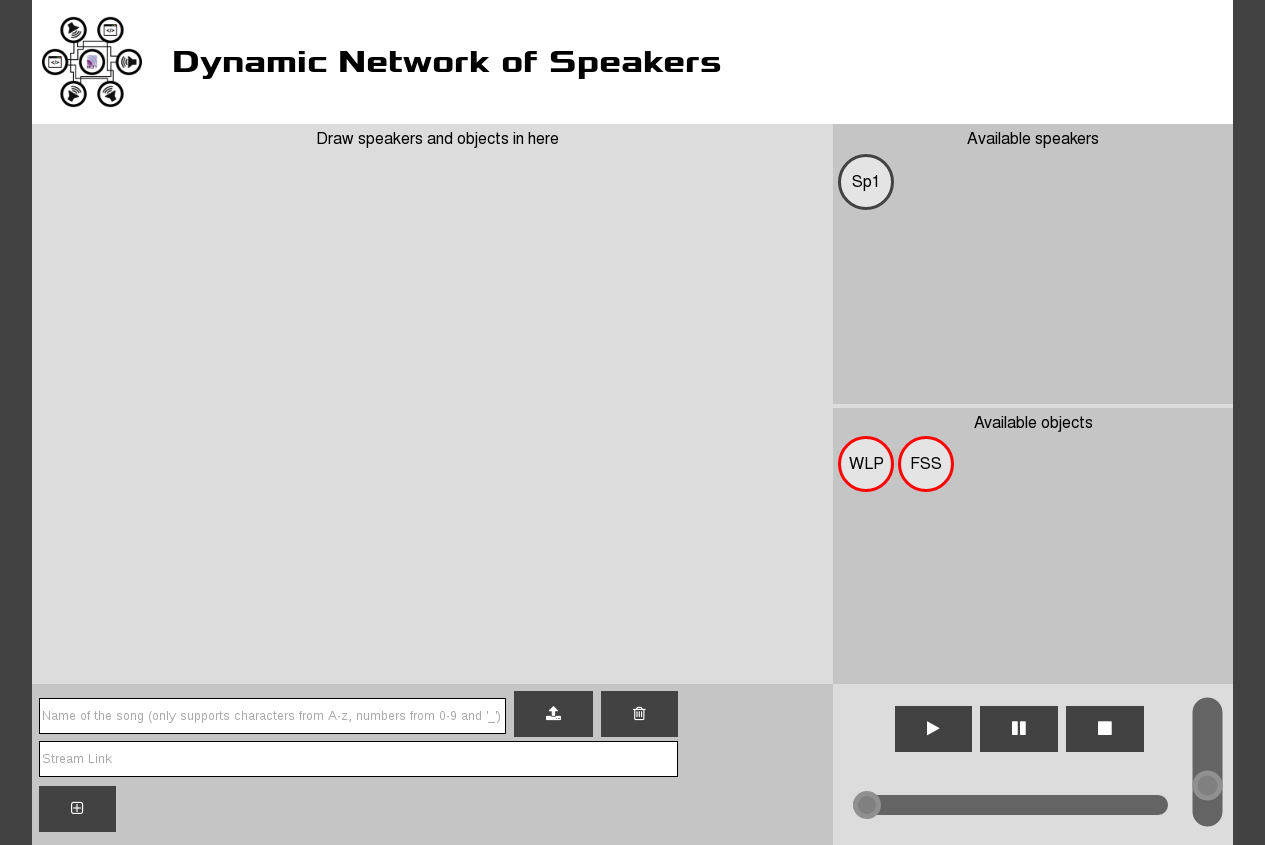
\includegraphics[width=.8\textwidth]{website_idle}
    \caption{Website when idle}
    \label{fig:website_idle}
\end{figure}

The following features are available:
\begin{shortlist}
    \item Available speakers list
    \begin{shortlist}
        \item Listing of all the online speakers
    \end{shortlist}
    \item Available object list
    \begin{shortlist}
        \item Listing off all the available objects
    \end{shortlist}
    \item Music controls (right bottom corner)
    \begin{shortlist}
        \item Music status control (play, pause, stop)
        \item Volume control
        \item Time playback control (not yet implemented)
    \end{shortlist}
    \item Object controls (left bottom corner)
    \begin{shortlist}
        \item Object name field
        \item URI field
        \item Upload button
        \item Delete button
    \end{shortlist}
    \item Extra controls (+ button)
    \begin{shortlist}
        \item See section about the \nameref{sub:website_Extra_options}
    \end{shortlist}
\end{shortlist}

\subsection{Manipulating speakers and objects}
\label{sub:manipulating_speakers_and_objects}
As shown in figure \ref{fig:website_1sp_2obj} and \ref{fig:website_2sp_2obj}, the speakers and objects can be dragged over to the draw area.
In this example there is first one speaker and two objects and in the second example there are two speaker and two objects.
As demonstrated here, the speakers and objects can simply be dragged around with the mouse.

The moment that there is a speaker available, e.g. a speaker comes online, it will show up in it's \say{available speakers} list.
From that moment, the user can simply drag the speaker to it's desired location.

\begin{figure}[H]
    \centering
        \begin{minipage}[b]{0.5\textwidth}
            \centering
            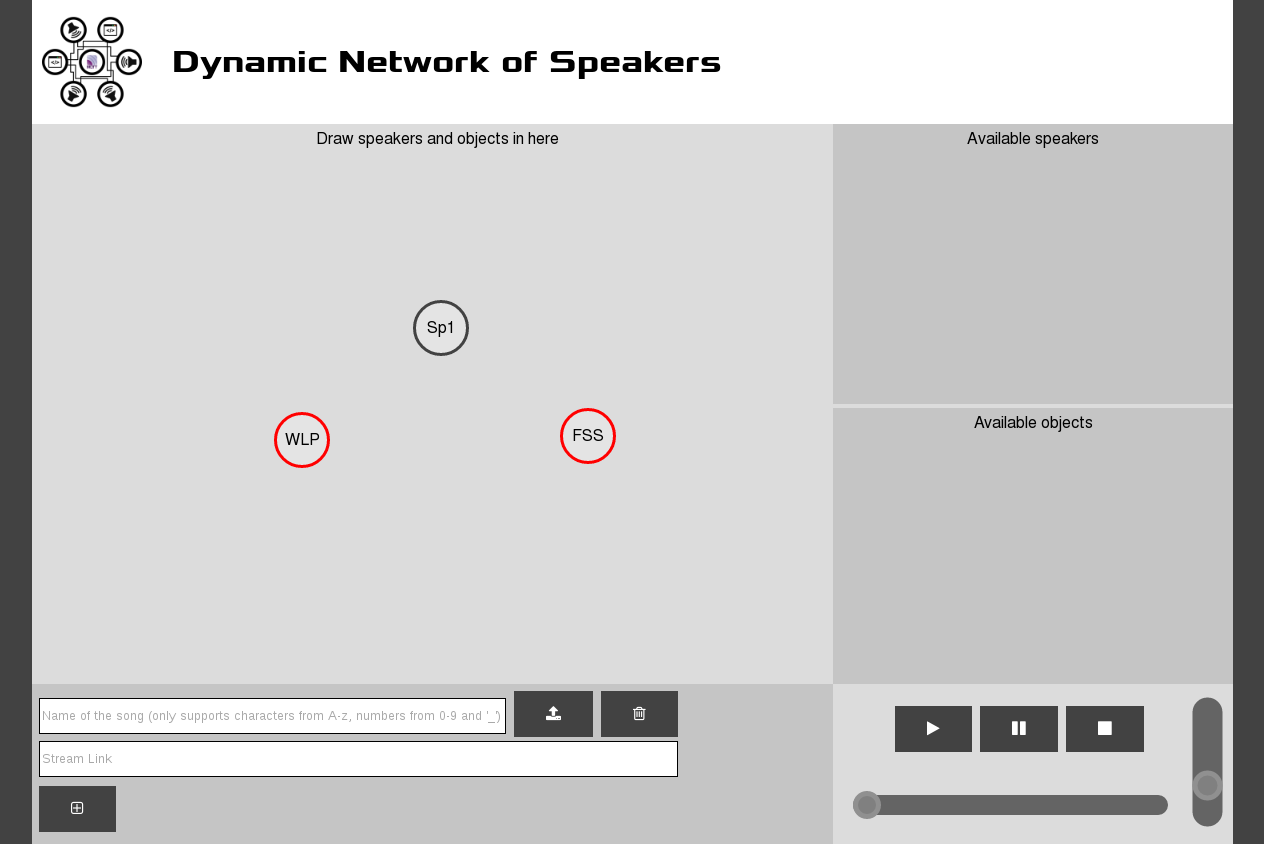
\includegraphics[width=.9\textwidth]{website_1sp_2obj}
            \caption{One speaker and two objects}
            \label{fig:website_1sp_2obj}
        \end{minipage}%
        %
        \begin{minipage}[b]{0.5\textwidth}
            \centering
            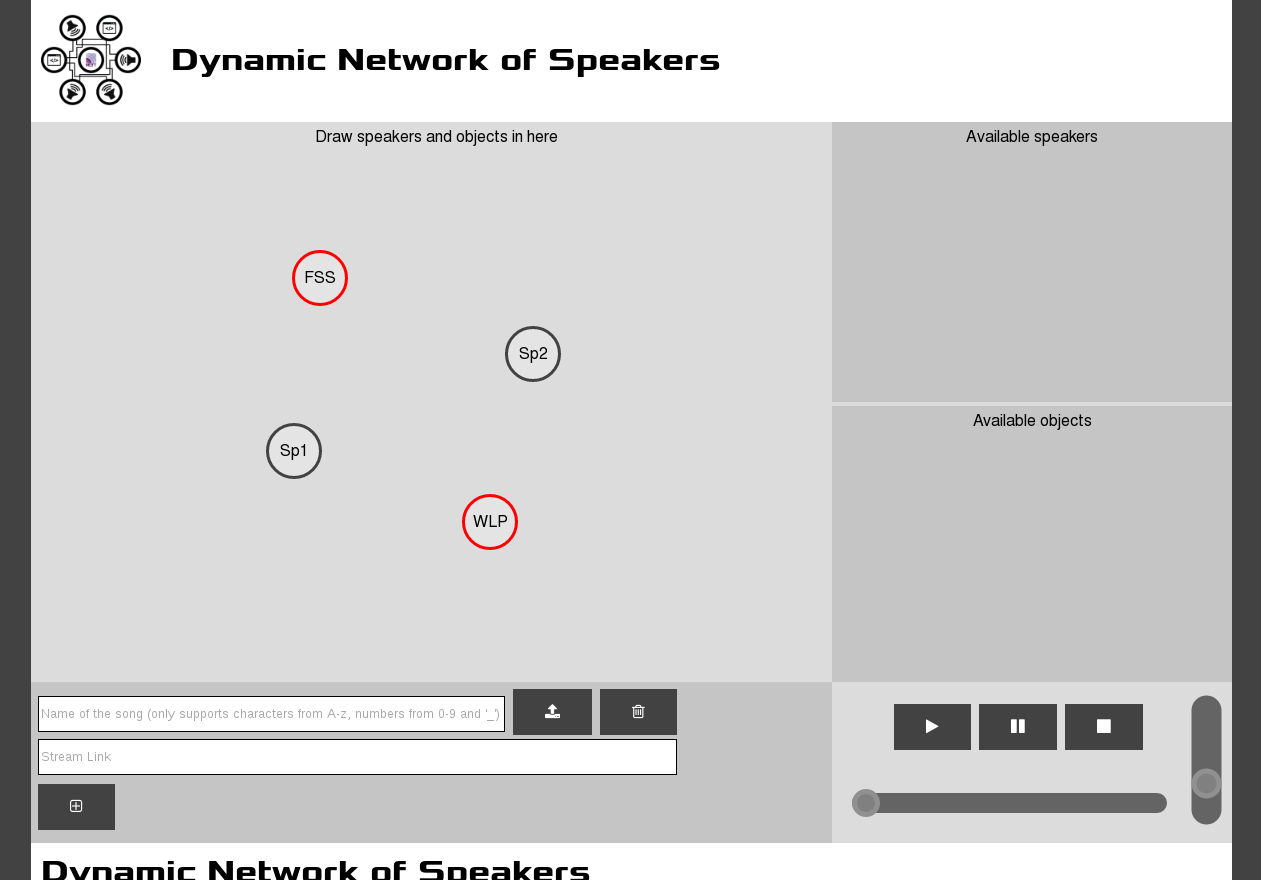
\includegraphics[width=.9\textwidth]{website_2sp_2obj}
            \caption{Two speakers and two objects}
            \label{fig:website_2sp_2obj}
    \end{minipage}
\end{figure}

\subsection{Edit objects}
\label{sub:website_edit_objects}
This website also has the ability to add, delete or modify any existing objects.
Figure \ref{fig:website_edit_object} shows this process.

\begin{figure}[H]
    \centering
    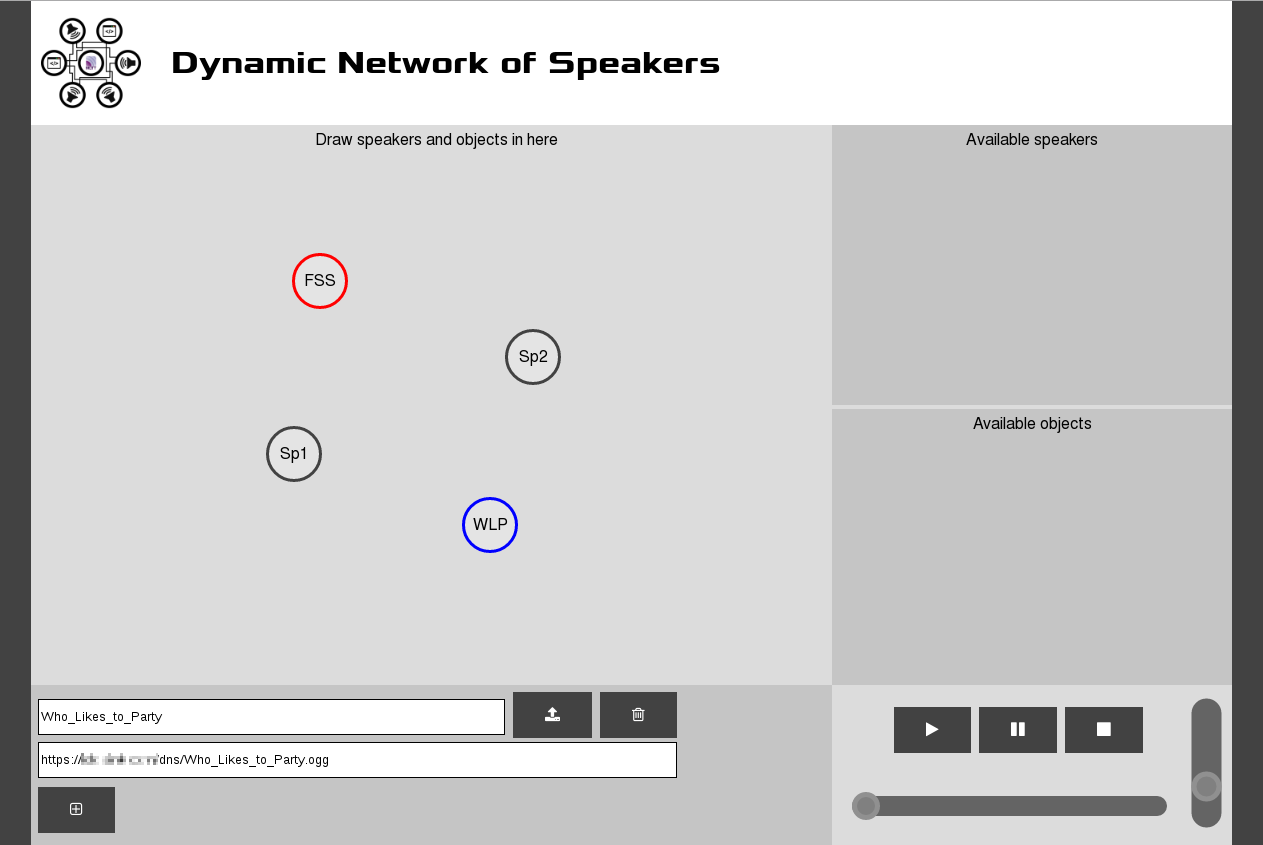
\includegraphics[width=.8\textwidth]{website_edit_object}
    \caption{Edit an object}
    \label{fig:website_edit_object}
\end{figure}

The following list will show the steps necessary to complete the listed actions.
\begin{shortlist}
    \item Add an object
    \begin{itemize}
        \item Fill in the Name of the object
        \item Fill in the URI of the object
        \item Press the upload button
    \end{itemize}
    \item Delete an object
    \begin{itemize}
        \item Select an object (the selected object is marked with a colored circle, blue in this case)
        \item Press the delete button
    \end{itemize}
    \item Modify an existing object
    \begin{itemize}
        \item Select an object (the selected object is marked with a colored circle, blue in this case)
        \item Modify the URI\footnote{Editing the name will result in uploading a new object with that name or overriding an object with that name}
        \item Press the upload button
    \end{itemize}
\end{shortlist}

\subsection{Extra options}
\label{sub:website_Extra_options}
The extra options tab, as shown in figure \ref{fig:website_extra_options}, holds some extra options that are not of a great importance for the main function of this site.

\begin{figure}[H]
    \centering
    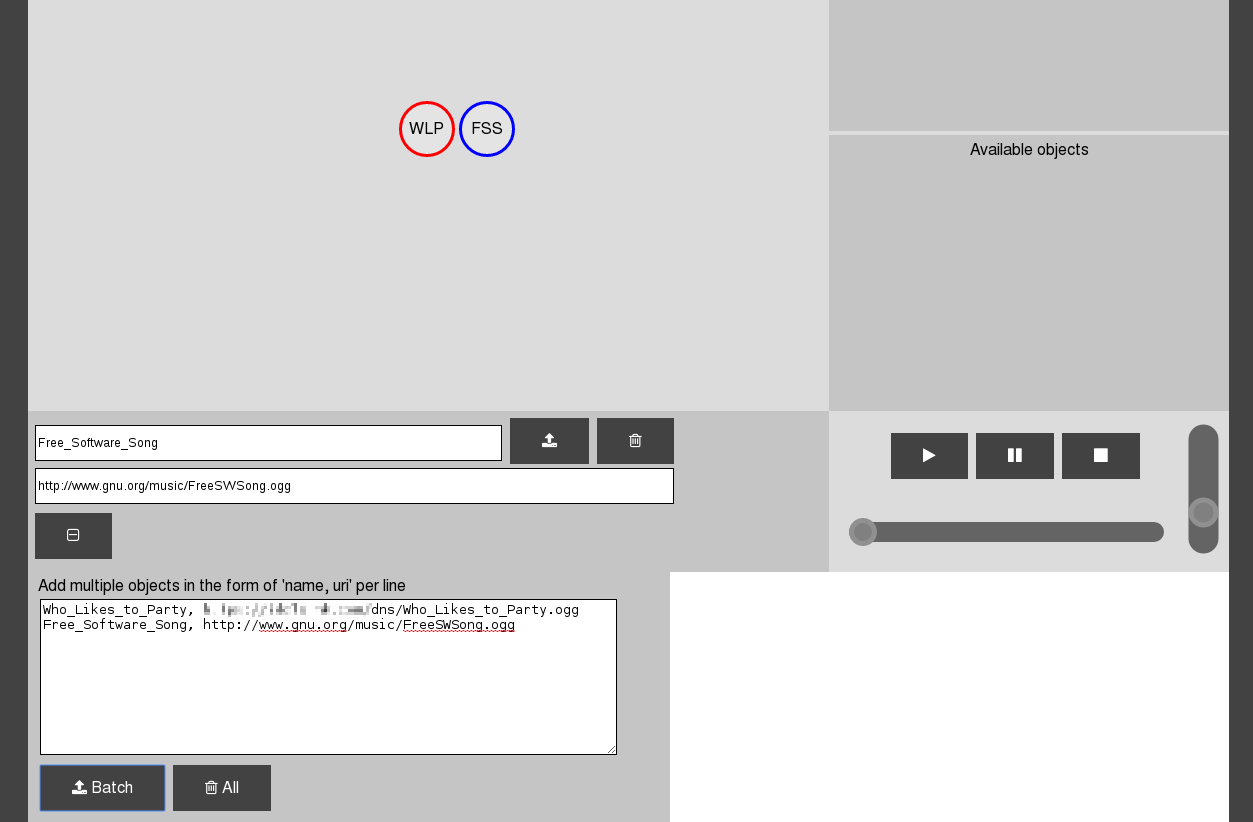
\includegraphics[width=.8\textwidth]{website_extra_options}
    \caption{Extra options}
    \label{fig:website_extra_options}
\end{figure}

This tab has the ability to batch upload and delete all objects.
This can be helpful when using this website in combination with multitrack\footnotemark songs and the user wants to upload multiple objects at once.
\footnotetext{A song split up into multiple stems. A single stem may be delivered in mono, stereo, or in multiple tracks for surround sound.}


    \chapter{Conclusion}            % Conclusion
    \label{chap:Conclusion}
    Conclusion: what is achieved?


    \clearpage      % Clear page for LoT
    \phantomsection % For hyperreflinking
    \addcontentsline{toc}{chapter}{\listtablename}  % Add LoT to ToC
    \listoftables                   % Generate and include a LoT
    %\thispagestyle{empty}           % Disable header and footer on LoT

    \clearpage      % Clear page for LoF
    \phantomsection % For hyperreflinking
    \addcontentsline{toc}{chapter}{\listfigurename} % Add LoF to ToC
    \listoffigures                  % Generate and include a LoF

    \printbibliography[heading=bibintoc] % Generate and include bibliography if needed
    %\thispagestyle{empty}           % Disable header and footer on bibliography

\end{document}
